\section{Calibration}
\label{sec:calib}

For accomplishing the object avoidance, it is essential to determine the position of the object with a reasonable accuracy. Since our stereo camera has a fixed position in the workcell and we need the position of the ball with respect to the robot, we needed to perform an eye-to-hand camera calibration process. Our main goal was to get a fairly accurate transformation from the camera to the base of the robot. After getting this transformation matrix, the result of the triangulation can be used (which is a translation vector from the camera frame) to obtain the position of the ball in the robot base frame.\\

There are multiple ways to perform this camera calibration. We chose to go a simple way, because eye-to-hand calibration was not our focus area. Also, it's not a huge problem if we have a relatively small error in the position of the ball because we are only doing avoidance and not something which requires more precise information, for example object grasping. Furthermore, we are adding some clearance to the constructed collision area to deal with the errors originating from the quick and easy calibration process.\\

Our method was to measure the distances along the coordinate axis of the robot base with a tape measure. This gave us a rough idea about the position of the camera with respect to the robot. The orientation required a bit more work. The idea was to add a simulated camera to the provided RobWork workcell and compare the image of it with the image of the left camera of the Bumblebee.\\

\begin{figure}[ht!]
    \centering
    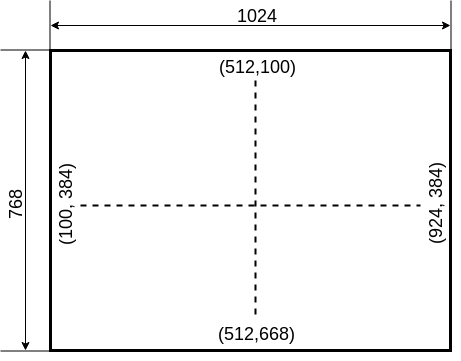
\includegraphics[width=0.6\textwidth]{Images/definedpoints.png}
    \caption{Defined cross on the image of the camera}
    \label{fig:definedpoints}
\end{figure}

We defined four points to define a cross on the picture of the left camera like on Figure \ref{fig:definedpoints}. \\

We moved the robot into such configurations where we had the TCP aligned with the defined points and recorded the 3D positions of the TCP. Afterwards, we placed four small objects into the recorded 3D positions in RobWorkStudio. We drew a cross to the picture of the simulated camera to help the alignment. The camera orientation was adjusted until we aligned the objects with the cross as good as possible.\\

\begin{figure}[ht!]
    \centering
    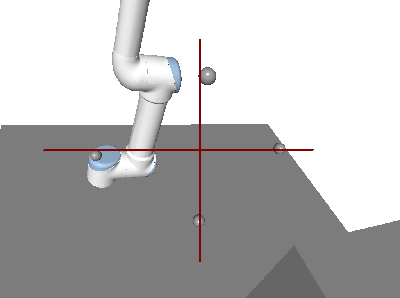
\includegraphics[width=0.6\textwidth]{Images/robwork_calib.png}
    \caption{Finding the right orientation of the camera with the help of a simulated camera in RobWorkStudio}
    \label{fig:robwork_calib}
\end{figure}

As a result, we obtained the Euler angles of the camera frame with respect to the robot base frame. We constructed a transformation matrix of these angles and the translation and inverted it using RobWork to get the final input for the triangulation program.